% !Mode:: "TeX:UTF-8"
%!TEX program = xelatex


\documentclass[a4paper, 10pt, twocolumn]{scrartcl}

% Mathematics
\usepackage{amsmath}
\usepackage{amssymb}
\usepackage{mathtools}
% \numberwithin{equation}{subsection}

% Font and Style
\usepackage{ucs}
\usepackage[T1]{fontenc}
\usepackage{abstract}
\usepackage{authblk}
\usepackage{url}
\usepackage{float}
\usepackage{hyperref}
\usepackage{indentfirst}
\usepackage{makecell}
\usepackage{booktabs}
\usepackage{listings}
\hypersetup{colorlinks=false}

% Font Package (select one)
\usepackage{lmodern}
% \usepackage{kpfonts}
% \usepackage{ccfonts}
%\usepackage{cmbright}
%\usepackage{antpolt}
% \usepackage{iwona}

\bibliographystyle{plain}

% Image and Graphics
\usepackage{graphicx}
\usepackage{dblfloatfix}
\usepackage[left=2.5cm, right=2.5cm, top=2.5cm, bottom=3cm]{geometry}
  \setlength{\columnsep}{15pt}

\newcommand{\bra}[1]{|{#1} \rangle}
\newcommand{\ket}[1]{\langle {#1}|}
\newcommand{\im}{\mathrm{i}}
\newcommand{\ee}{\mathrm{e}}
\newcommand{\I}{\begin{pmatrix*}[r] 1 &  0 \\ 0 & 1 \end{pmatrix*}}
\newcommand{\X}{\begin{pmatrix*}[r] 0 &  1 \\ 1 & 0 \end{pmatrix*}}
\newcommand{\Y}{\begin{pmatrix*}[r] 0 &  -\im \\ \im & 0 \end{pmatrix*}}
\newcommand{\Z}{\begin{pmatrix*}[r] 1 &  0 \\ 0 & -1 \end{pmatrix*}}
\newcommand{\Had}{\frac{1}{\sqrt{2}} (X+Z) = \begin{pmatrix*}[r] 1 &  1 \\ 1 & -1 \end{pmatrix*}}
\newcommand{\qubit}{\begin{pmatrix*}[r] a\\b \end{pmatrix*}}
\newcommand{\CNOT}{\begin{pmatrix*}[r] 1 & 0 & 0 & 0 \\ 
                                       0 & 1 & 0 & 0 \\
                                       0 & 0 & 0 & 1 \\
                                       0 & 0 & 1 & 0 \end{pmatrix*}}

\renewcommand*{\Authand}{\quad}
\renewcommand{\abstractname}{}
\renewcommand{\absnamepos}{empty}
\renewcommand\Affilfont{\fontsize{9}{10.8}\itshape}
\renewcommand\Authfont{\fontsize{12}{14.4}\selectfont}
% Document Information
\title{Implementation and Simulation of \\ Quantum Teleportation}
% \subtitle{Further specification goes here}
\author[*]{Student: Chen Xin}
\author[*]{Advisor: Li-Xiang Cen}
\affil[*]{\emph{College of Phsical Science and Technology, Sichuan University}}
\date{\vspace{-7ex}}



\begin{document}
  % Create Title, Abstract and TOC
  \twocolumn[\maketitle \begin{abstract} \centering \begin{minipage}{1.0\linewidth}
  The basic principle of quantum teleportation (QT) is reviewed first in the introduction, 
  and then some simple quantum gates which are necessary for QT are introduced in section 1. Next in section 2, we clarify how one could construct and measure a Bell state and relevant quantum circuits are illustrated. Finally, with all conceptions clear, 
  a program for simulation of QT is shown to testify the quantum circuit really works.


  \vspace{0.8cm}
  \end{minipage}\end{abstract}]
  % \tableofcontents

  % CONTENT
  \section*{Introduction}

	Quantum Teleportation (QT) appeared as a very fundamental but interesting topic in quantum information theory (QIT). The theory of QT was first published in 1993 by six scientists including Bennett\cite{art:93Bennett}. 
	According to their report, two qubits which form an EPR pair and a classic channel 
	can be used to teleport another qubit from Alice to Bob (named for a comventional reason).

	\begin{figure}[H]
	\centering
	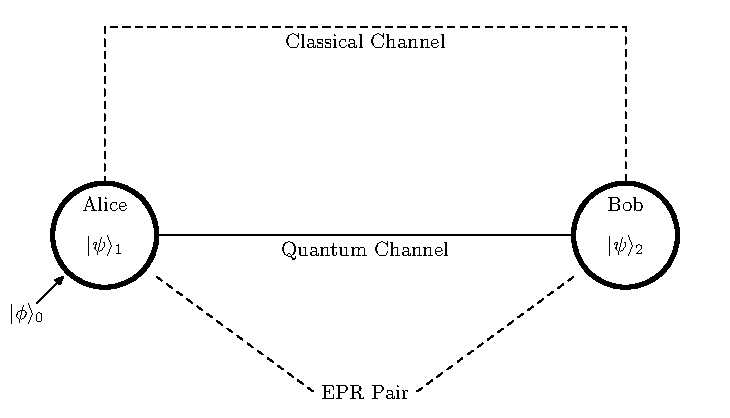
\includegraphics[scale=0.65]{img/QT-1.pdf}
	\caption{Quantum Teleportation}
	\label{img:QT}
	\end{figure}
	The whole system for this teleportation is shown in figure (\ref{img:QT}). Suppose that two qubits with 
	label $1,\ 2$ controlled by Alice and Bob respectively, form an EPR pair (or Bell state):
	\begin{equation}
	\bra{\psi}_{12} = \frac{1}{\sqrt{2}} (\bra{0}_1 \bra{1}_2 - \bra{1}_1  \bra{0}_2),
	\end{equation}
	which is used as a quantum channel and the distance between Alice and Bob can be any value.
	The task of this teleportation is to send another qubit 
	\begin{equation}
	\bra{\phi}_0 = a\bra{0}_0+b\bra{1}_0
	\end{equation} 
	from Alice to Bob (Alice could know nothing about $\bra{\phi}_0$). To complete this task, 
	Alice put $\bra{\phi}_0$ in her box together with qubit $1$, yielding a tri-qubit state in the whole system:
	\begin{equation}
	\label{eq:triQubit} 
		\begin{split}
		\bra{\psi}_{012} = &\frac{a}{\sqrt{2}} ( \bra{011} - \bra{100} )\\
						& + \frac{b}{\sqrt{2}} (\bra{011} - \bra{101}).
		\end{split}
	\end{equation}
	Next, using some apparatus, Alice
	measures and identifies which Bell state the pair $0\  \&\  1$ are at. To clarify this, 
	we should rewrite formula (\ref{eq:triQubit}) by projecting them to the four Bell states of qubits $0,1$ 
	\begin{equation}
	\label{eq:jointBell}
		\begin{aligned}
		\bra{\psi}_{012} = &\frac{1}{2} \Bigl[ \bra{\psi^-}_{01}(-a \bra{0}_2 - b \bra{1}_2 )\\
						 &+ \bra{\psi^+}_{01} (-a \bra{0}_2 +b \bra{1}_2)\\
						 &+ \bra{\phi^-}_{01} (a \bra{1}_2 + b \bra{0}_2)\\
						 &+ \bra{\phi^+}_{01} (a\bra{1}_2 -b \bra{0}_2) \Bigr].
		\end{aligned}
	\end{equation}
	So when Alice performs the measurement, $\bra{\psi}_{123}$ will collapse to one of the four parts 
	of right hand of equation (\ref{eq:jointBell}) with identical probabilities $1/4$.
	Meanwhile, when Bob detects qubit $2$, he will get the corresponding state 
	which can be restored to $\bra{\phi}_0$ by a unitary transformation. 
	To know this unitary transformation, Alice need to 
	tell Bob what is the Bell state of qubit $0 \& 1$ she obtained just now, 
	through the classical channel. For example, if Alice obtains $\bra{\psi^-}_{01}$, 
	then the state that Bob gets must be $-a \bra{0}_2 - b \bra{1}_2$ or $[-a, -b]$.
	After receiving Alice's information through classical channel, Bob can then restore qubit $0$ by
	\begin{equation}
	 \begin{pmatrix*}[r] a\\b \end{pmatrix*} =\begin{pmatrix*}[r] -1 &  0 \\ 0 & -1 \end{pmatrix*}
	 \begin{pmatrix*}[r] -a\\-b \end{pmatrix*}.
	\end{equation}

	Note that because the classical channel is necessary, information can not be transported at speed
	beyond light, even though the collapsing occurs at both sides instantaneously (a common theory).

	Above is just a basic and rough description of QT. There are 2 problems remaining: 
	a) how to generate an EPR pair; b) how to measure (identify) a Bell state. 
	To clarify these issues, knowledge about Quantum Gate, which will be introduced in next section.
	Because matrix operations can be perfomed conveniently in a computer, 
	a numerical simulation will be shown in the last section.

\section{Quantum Gates}
	\subsection{Quantum Gates for Single Qubit}
		A Quantum gate is a unitary operator for qubit(s), which can be represented, for single qubit, as a $2\times 2$ matrix. Such operators are all composed of Pauli matrices and are all reversible. Based on Pauli matrices, some simple quantum gates can be formed
		\begin{equation}
		\begin{split}
		&I = \I,\  
		 X = \X \\
		&Y = \Y,\ 
		 Z = \Z\\
		&H = \Had.
		\end{split}
		\end{equation}

		Given a qubit $\bra{phi} = a\bra{0} + b\bra{1}$, it is easy to check
		\begin{align}
		I \bra{\phi} &= a\bra{0} + b\bra{1} \\
		X \bra{\phi} &= b\bra{0} + a\bra{1}\\
		Y \bra{\phi} &= -\im b\bra{0} + \im a\bra{1}\\
		Z \bra{\phi} &= a\bra{0} - b\bra{1}\\
		H \bra{\phi} &= \frac{1}{\sqrt{2}} \Bigl[ a(\bra{0}+\bra{1})+b(\bra{0}-\bra{1}) \Bigr] \notag \\
		&= a \bra{+}+b\bra{-}.
		\end{align}
		where $X,Y,Z$ are just Pauli matrices $\sigma_x,\sigma_y,\sigma_z$ respectively, and $H$ is Hadamard\cite{art:Hardamard} matrix gate which can transform any qubit into a superposition state $a \bra{+}+b\bra{-}$. We will use $H$ to construct EPR pair later.
		\begin{figure}[H]
		\centering
		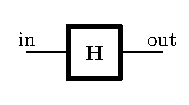
\includegraphics[scale=1.2]{img/singleGate-1.pdf}
		\caption{Quantum gate for a single qubit.}
		\label{img:1qubitGate}
		\end{figure}
		A gate for a single qubit has one input and one output. 
		An example is illustrated in figure (\ref{img:1qubitGate}).

	\subsection{CNOT Gate}
		CNOT stands for Controlled NOT gate with a control terminal $a$ and a target terminal $x$. 
		In classical circuits, $a$ and $x$ is certainly $0$ or $1$. $x$ holds the value when $a=0$ and becomes $\bar{x}$ (NOT $x$) when $a=1$. In a word, $x$ is always left $x$XOR$a$ after a CNOT gate with control bit $a$.

		In the quantum situation, the difference is that both $\bra{a}$ and $\bra{x}$ 
		(Dirac notation for quantum) can be some superposition states, but the 
		basic idea of CNOT is the same as a classical one.
		Two typical kinds of inputs and outputs are shown in figure (\ref{img:CNOT}).
		\begin{figure}  
		\centering
		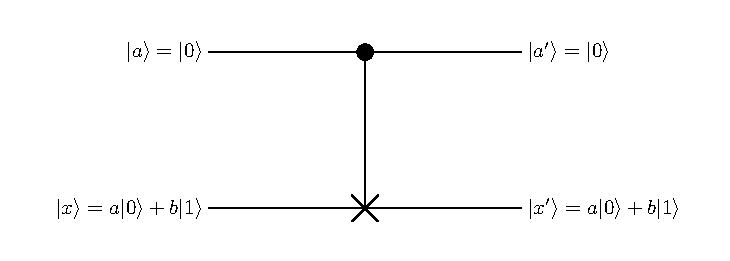
\includegraphics[scale=0.7]{img/CNOT-1.pdf}
		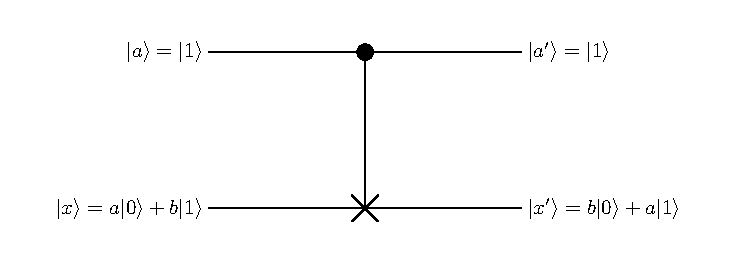
\includegraphics[scale=0.7]{img/CNOT-2.pdf}
		\caption{CNOT gate with control qubit $\bra{a}$ and target qubit $\bra{x}$.}
		\label{img:CNOT}
		\end{figure}
		Note that the two lines in figure (\ref{img:CNOT}) represented for 
		qubits $\bra{a}$ and $\bra{x}$ can also be entangled, so it is better to find the $2\times 2$ matrix representation of CNOT for convenience.

		The direct product of $\bra{a}$ and $\bra{x}$ can be written as a 4D vector
		\begin{equation} 
			\begin{split}
			\bra{a}\otimes\bra{x} &= u_1\bra{00} +u_2\bra{01}\\
				&\quad+u_3\bra{10}+u_4\bra{11}\\
				&=\begin{pmatrix*}[r] u_1\\u_2\\u_3\\u_4 \end{pmatrix*},
			\end{split}
		\label{eq:BeforeCNOT}
		\end{equation}
		where the direct product symbol "$\otimes$" is omitted at right hand.
		And the "XOR idea" is also available here, which means 
		$\bra{a,x} \mapsto \bra{a,a\ \text{XOR}\ x}$ under a CNOT operation. 
		Let $A_{\text{CNOT}}$ be the matrix of CNOT, then
		\begin{equation}
			\begin{split}
			A_{\text{CNOT}} \bra{a}\otimes\bra{x} &= u_1\bra{00} +u_2\bra{01}\\
				&\quad+u_3\bra{11}+u_4\bra{10}\\
				&=\begin{pmatrix*}[r] u_1\\u_2\\u_4\\u_3 \end{pmatrix*}.
			\end{split}
		\label{eq:AfterCNOT}
		\end{equation}

		Now it's easy to find the matrix transforming 
		the vector in equation (\ref{eq:BeforeCNOT}) to that in equation (\ref{eq:AfterCNOT}), 
		which just keeps $u_1,\ u_2$ unchanged and makes $u_3,\  u_4$ swaped:
		\begin{equation}
		A_{\text{CNOT}}= \CNOT.
		\end{equation}

\section{Realization of Quantum Teleportation}
	With quantum gates, we can build, like the classical logic circuit, quantum circuit.
	In this section, kinds of quantum circuits are introduced, 
	which can make QT come true step by step.
	\subsection{Constructing Entangled Pairs}
		\label{subsec:CstEP}
		Consider the general situation of a CNOT gate, i.e. inputs 
		with two qubits which are both at superposition states, as shown in figure (\ref{img:CNOTGeneral}).
		\begin{figure}
		\centering
		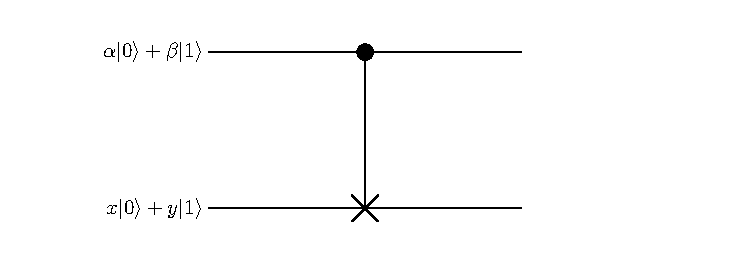
\includegraphics[scale=0.7]{img/CNOT-3.pdf}
		\caption{CNOT with two superposition states as inputs.}
		\label{img:CNOTGeneral}
		\end{figure}
		Because the outcome may be a entangled pair, we can not treat the two lines separately, which requires us calculate the outcome in a direct product form:
		\begin{equation}
			\begin{split}
			A_{\text{CNOT}}&(\alpha \bra{0}+\beta\bra{1})\otimes (x\bra{0}+y\bra{1}) \\
			&= \CNOT \begin{pmatrix*}[r] \alpha x\\ \alpha y \\ \beta x \\ \beta y \end{pmatrix*}\\
			&= \begin{pmatrix*}[r] \alpha x\\ \alpha y \\ \beta y \\ \beta x \end{pmatrix*}
			\end{split}
			\label{eq:CNOT_outcome}
		\end{equation}
		Note that the two qubits of inputs are separable. 
		Now we shall ask "in what situation should the outcome be entangled?". Rewrite 
		the outcome in formula (\ref{eq:CNOT_outcome}) as 
		\begin{equation}
		\begin{bmatrix*}[r] \alpha \begin{pmatrix*}[r] x \\ y \end{pmatrix*}\\
							\beta \begin{pmatrix*}[r] y \\ x \end{pmatrix*} 
							\end{bmatrix*}.
		\end{equation}
		It is seen that if $\alpha \neq 0$, $\beta \neq 0$ (namely the control qubit is 
		a superposition state) and $x \neq y$, than the outcome can not be decomposited
		into direct product, which means an entangled outcome.

		So the conclusion is that we can use a CNOT with a control qubit at superposition state 
		to construct entangled pairs. We already know Hadamard gate generate 
		superposition state, so a quantum circuit\cite{book:IT} for constructing entangled 
		pairs can be built, as shown in figure (\ref{img:constructEntangle}).
		\begin{figure}
		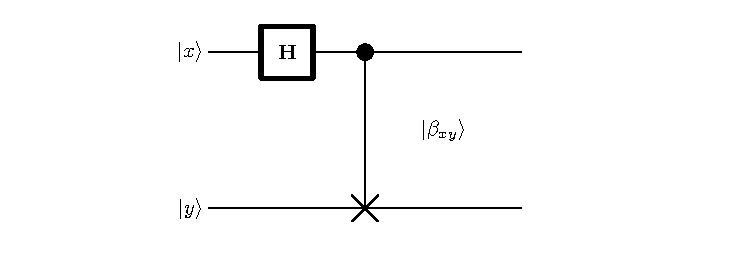
\includegraphics[scale=0.7]{img/entangled_pair-1.pdf}
		\caption{Quantum circuit for constructing entangled pair.}
		\label{img:constructEntangle}
		\end{figure}

		The notation $\bra{\beta_{ax}}$ is for Bell states:
		\begin{align}
		\bra{\beta_{00}} = \frac{1}{\sqrt{2}} (\bra{00}+\bra{11})\\
		\bra{\beta_{01}} = \frac{1}{\sqrt{2}} (\bra{01}+\bra{10})\\
		\bra{\beta_{10}} = \frac{1}{\sqrt{2}} (\bra{00}-\bra{11})\\
		\bra{\beta_{11}} = \frac{1}{\sqrt{2}} (\bra{10}-\bra{01})
		\end{align}
		We will see these binary encoding for Bell states exactly show the corresponding
		relation between the input and outcome of the circuit. For example, inputs 
		$\bra{a} = \bra{0},\ \bra{x}=\bra{0}$ lead to the outcome $\bra{\beta_{00}}$, and it's convenient to check the others.

	\subsection{Measuring Bell States}
		As mentioned in Instruction, in a QT system, Alice need some apparatus to 
		identify which Bell state qubit $0\ \& 1$ are at. 
		We have seen, in subsection \ref{subsec:CstEP}, inputs with two separable qubits
		lead to an entangled outcome. In turn, we will soon check, an input with an entangled pair for the inverse circuit leads to a separable pair.
		\begin{figure}
		\centering
		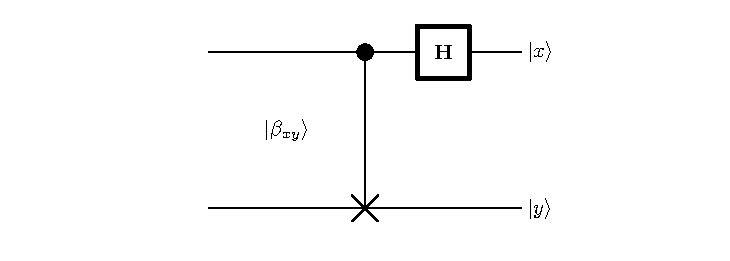
\includegraphics[scale=0.7]{img/separable_pair-1.pdf}
		\caption{Quantum circuit for separating an entangled pair.}
		\label{img:separateEntangle}
		\end{figure}

		Figure (\ref{img:separateEntangle}) shows the inverse version of figure (\ref{img:constructEntangle}). This can be checked as follows. Suppose an entangled input, say
		 $\bra{\beta_{00}}$. CNOT acts on it first:
		\begin{equation}
		\begin{split}
			A_{\text{CNOT}} \bra{\beta_{00}} &= A_{\text{CNOT}} \frac{1}{\sqrt{2}} (\bra{00}+\bra{11})\\
			&=\frac{1}{\sqrt{2}} (\bra{00}+\bra{10}),
		\end{split}
		\end{equation}
		then the Hadamard follows. Note that because the Hadamard lives in a subspace of the whole direct space, we need to make a direct product with an identity matrix on it before acting it on the entangled pair:
		\begin{equation} 
		\begin{split}
			&\ (H\otimes I) \frac{1}{\sqrt{2}} (\bra{00}+\bra{10})\\
			=& \frac{1}{\sqrt{2}} (\bra{+0}+\bra{-0})\\
			=&\frac{1}{2}(\bra{00}+\bra{01}+\bra{00}-\bra{01})\\
			=&\bra{00} = \bra{0}\otimes\bra{0}.
		\end{split}
		\end{equation}
		As you can see, the outcome is a separable pair and each qubit of the pair is at
		an eigenstate, which means if we measure each line of the outcome, we will get
		eigen values $0$ and $0$ respectively. 
		See the binary encoding always matches with the Bell states. Outcomes of other entangled inputs can be checked in the same way.

	\subsection{The Entire Circuit}
		Now we are in the position to build the entire circuit for QT. 

		Assemble the quantum gates introduced before following figure 
		(\ref{img:entireCircuit}). 
		\begin{figure}
		\centering
		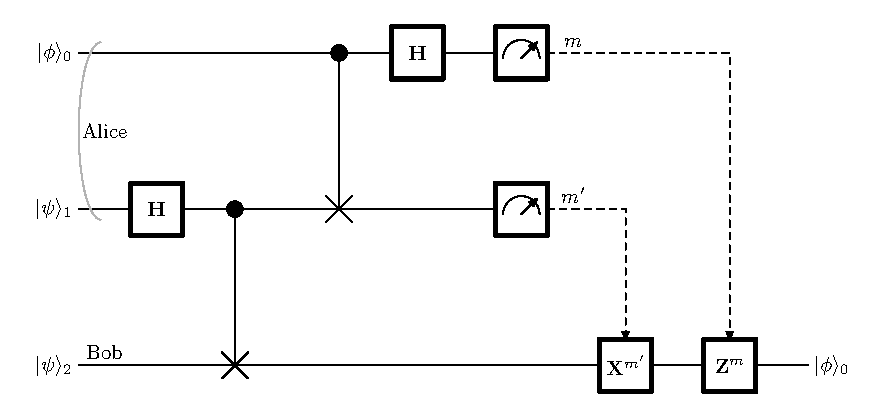
\includegraphics[scale=0.6]{img/EntireCircuit-1.pdf}
		\caption{Entire circuit for QT.}
		\label{img:entireCircuit}
		\end{figure}
		As shown in figure, Bob controls $\bra{\psi}_2$ and Alice controls the other two
		qubits. Let $\bra{\phi}_0 = a\bra{0}+b\bra{b}$ be the qubit 
		waiting for teleportation.

		The first part is the entangled-pair-constructor at the left bottom. 
		Let the inputs $\bra{\psi}_1 = \bra{0}$ and $\bra{\psi}_2=\bra{0}$, then 
		$\bra{\beta_{00}}_{12}$ is yielded\footnote{
		All of the four Bell states can be used in QT, while different choice leads to 
		different unitary matrix that Bob uses to restore $\bra{\phi}_0$.}.  
		Next, Alice add $\bra{\phi}_0$ to the system, making the system a tri-qubit
		\begin{equation}
			\begin{split}
			&\bra{\phi}_0 \otimes \bra{\beta_{00}}_{12} \\
				=&(a\bra{0}+b\bra{1}) \otimes \frac{1}{\sqrt{2}} (\bra{00}+\bra{11})\\
				=&\frac{1}{\sqrt{2}} (a\bra{000}+a\bra{011}+b\bra{100}+b\bra{111}),
			\end{split}
		\end{equation}
		which is a 8D vector.

		Next part at right top is for Alice to identify Bell states for $\bra{\psi}_{01}$. The icons like gauge meters stand for measurement apparatus. After the operation of CNOT, the tri-qubit becomes (use "XOR idea")
		\begin{equation}
		\frac{1}{2}(a\bra{000}+a\bra{011}+b\bra{110}+b\bra{101}).
		\end{equation}
		The Hadamard in this part acts on qubit $0$, and the result is easy to obtained:
		\begin{equation} 
			\begin{split}
				\frac{1}{2}[&a\bra{000}+a\bra{100}+a\bra{011}+a\bra{111}\\
						&+b\bra{010}-b\bra{110}+b\bra{001}-b\bra{101}],
			\end{split}
		\end{equation}
		or (because direct product satisfies distributive law):
		\begin{equation}
		\label{eq:final}
		\begin{split}
		 &\bra{00}_{01}\frac{a\bra{0}_2+b\bra{1}_2}{2} +\bra{01}_{01}\frac{b\bra{0}_2+1\bra{1}_2}{2} \\
		 +&\bra{10}_{01}\frac{a\bra{0}_2-b\bra{1}_2}{2}+\bra{11}_{01}\frac{-b\bra{0}_2+a\bra{1}_2}{2} .
		 \end{split}
		\end{equation}
		Notice that the $\bra{00}_{01},\ \bra{01}_{01},\ \bra{10}_{01},\ \bra{11}_{01}$ in equation \ref{eq:final} generated from Alice's apparatus are not, but corresponding to Bell states 
		$\bra{\beta_{00}}_{01},\ \bra{\beta_{01}}_{01},\ \bra{\beta_{10}}_{01},\ \bra{\beta_{11}}_{01}$ respectively. After Alice's measurement the tri-qubit will collapse into one of the 
		four items in equation (\ref{eq:final}) with equivalent probabilities. 

		Finally, Bob uses $X^{m'}$ gate and $Z^{m}$ gate to restore $\bra{\phi}_0$. $m$ and $m'$ 
		stand for Alice's measurement result, corresponding to Bell state $\bra{\beta_{mm'}}_{01}$, 
		and Bob is told this result through classical channel. Next Bob acts matrix $Z^{m}X^{m'}$ on
		qubit $2$, then he will restore the $\bra{\phi}_0$. All situations are listed in table (\ref{tab:measure}).
		\begin{table}
		\centering			\begin{tabular}{c c c c c}
			\toprule
			m  &  m' &  Alice           &  Bob      &  $Z^{m}X^{m'}$ \\
			\midrule
			0  &  0  &  $\bra{00}$      &  $a\bra{0}+b\bra{1}$  &  $I$ \\
			0  &  1  &  $\bra{01}$      &  $b\bra{0}+a\bra{1}$  &  $X$ \\
			1  &  0  &  $\bra{10}$      &  $a\bra{0}-b\bra{1}$  &  $Z$ \\
			1  &  1  &  $\bra{11}$      &  $-b\bra{0}+a\bra{1}$ &  $ZX$ \\
			\bottomrule
			\end{tabular}
			\caption{Relations between Alice and Bob's measurement. After Alice's measurement, Bob can restore $\bra{\phi}_0$ in his qubit $2$ with corresponding matrix.}
			\label{tab:measure}
		\end{table}

\section{Simulation for QT}
	At last a program will be introduced here for testifying the theory of QT. I coded with Python 
	and the program just follows the process shown in figure (\ref{img:entireCircuit}).

	In my simulation, normalized $\bra{\phi}_0$s are generated randomly. And pseudo-random numbers are used to simulate collapsing. One simulation result 
	are shown as follow.
	\begin{figure}[H]
	\centering
	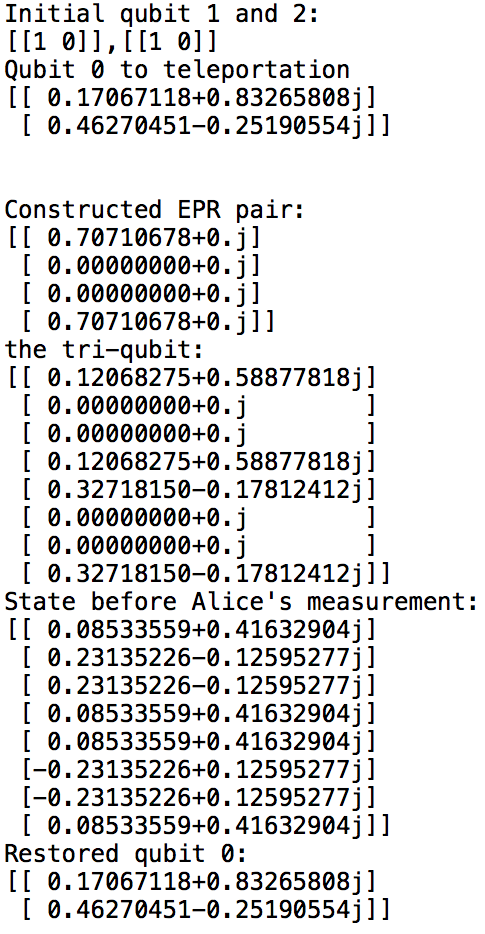
\includegraphics[width=5cm]{img/simRes.png}
    \end{figure}
    As shown above, the restored qubit $0$ is exactly the same as the original one, which means the quantum circuit does work well.
    Because there are no quantum things really happens, 
    this is just a toy program for fun\footnote{
    The code is uploaded to https://github.com/Varato/QT\_sims}.
     
\section*{Summary}
	As the program testified, if neglecting decoherence, QT works very well. 
	This provides a way to send a quantum state from one to one. 
	It is worth mentioning that classical and quantum channel are both necessary for QT.
	Only quantum channel can not transmit any information. It can be explained as follows:
	\begin{enumerate}
	\item The amount of information Bob can obtain when measuring his qubit depends on 
	the partial entropy of entanglement (equals 1 for Bell state), and Alice's local measurement can not cause any change of this entropy. Further to say, qubit $2$ is in a mixed state for Bob who can only access qubit $2$ until he measures it.
	\item It is believed collapsing is instantaneous and nonlocal, which means Bob's qubit
	can response Alice's measurement without any delay, while transmission of
	information faster than light is not physical. This also ensures that along the 
	quantum channel, no one other than Alice and Bob could fetch the quantum state of  qubit $0$.
	\end{enumerate}
	And Through the classical channel, only part of information can Alice transmit to Bob, which means even though the classical information is eavesdropped, without Bob's
	qubit, the eavesdropper can not fetch the qubit $0$ ether. This feature provide a scheme for Quantum private key distribution (QKD)\cite{art:QKD}. 

	Because  noise and decoherence are all neglected in the theory and simulation above, so we are still far away from the real physical situation.














  % Input your source files here
  % Bibliography
  \bibliography{bib/bibliography.bib}
\end{document}
